\chapter{Формулы Грина.}
\label{cha:15}

\begin{theorem}[\blue{Формула Гаусса - Остроградского}]
	Для функции $w$ имеем следующую формулу:
	\begin{multicols}{2}

			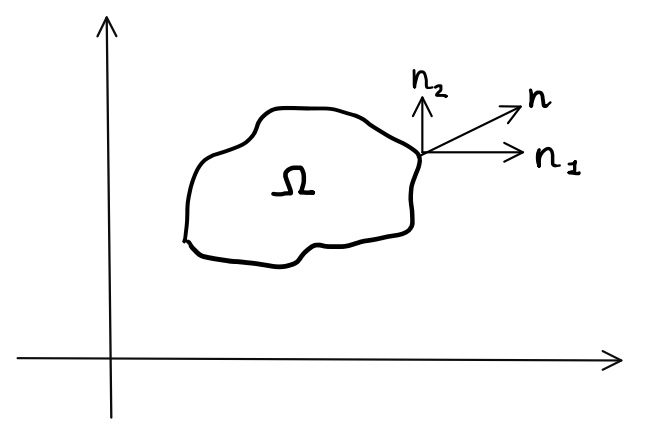
\includegraphics[scale = 0.3]{cha15im1}
		\columnbreak

			\hfill \break
			$$\underset{\Omega}{\int\int} \dfrac{\partial \omega}{\partial x_i}d\bar{x} = \oint\limits_{\partial \Omega} \omega n_i d\sigma$$
	\end{multicols}
\end{theorem}

\begin{theorem}[\blue{Многомерная формула интегрирования по частям}]
	Для функции $ \omega = uv $ имеем следующую формулу:
	$$\begin{gathered}
		\underset{\Omega}{\int\int} u \dfrac{\partial v}{\partial x_i}d\bar{x} = \oint\limits_{\partial \Omega} u v n_i d\sigma - \underset{\Omega}{\int\int} v \dfrac{\partial u}{\partial x_i}d\bar{x}.
	\end{gathered}$$
\end{theorem}

\begin{theorem}[\blue{I формула Грина}]
	Для функции $ \omega = u \dfrac{\partial v}{\partial x_i} $ имеем следующую формулу:
	$$\begin{gathered}
		\underset{\Omega}{\int\int} u \dfrac{\partial^2 v}{\partial x^2_i}d\bar{x} = \oint\limits_{\partial \Omega} u \dfrac{\partial v}{\partial x_i} n_i d\sigma - \underset{\Omega}{\int\int} \dfrac{\partial u}{\partial x_i} \dfrac{\partial v}{\partial x_i} d\bar{x} \mid \sum\limits_{i = 1}^k \Longrightarrow \\
		\Longrightarrow \underset{\Omega}{\int\int} u \Delta v d \bar{x} = \oint\limits_{\partial \Omega} u \dfrac{\partial v}{\partial \bar{n}}d\sigma - \underset{\Omega}{\int\int} (\bar{\nabla}u, \bar{\nabla}v)
		d\bar{x}
	\end{gathered}$$
\end{theorem}\newpage

\begin{theorem}[\blue{II формула Грина}]
$$
\begin{gathered}
\underset{\Omega}{\int\int} v \Delta u d\bar{x} = \oint\limits_{\partial \Omega} v \dfrac{\partial u}{\partial \bar{n}} d\sigma - \underset{\Omega}{\int\int} (\bar{\nabla}v, \bar{\nabla}u)d\bar{x} \\
- \\
\underset{\Omega}{\int\int} u \Delta v d \bar{x} = \oint\limits_{\partial \Omega} u \dfrac{\partial v}{\partial \bar{n}}d\sigma - \underset{\Omega}{\int\int} (\bar{\nabla}u, \bar{\nabla}v)d\bar{x} \\
= \\
\underset{\Omega}{\int\int} (u \Delta v - v \Delta u)d\bar{x} = \oint\limits_{\partial \Omega} (u \dfrac{\partial v}{\partial \bar{n}} - v \dfrac{\partial u}{\partial \bar{n}})d\sigma.
\end{gathered}
$$
\end{theorem}

\begin{theorem}[\blue{Теорема о потоке}]
	Если $ \omega = \dfrac{\partial u}{\partial x_i}$, то справедлива формула:
	$$\begin{gathered}
		\underset{\Omega}{\int\int} \Delta u d\bar{x} = \oint\limits_{\partial \Omega} \dfrac{\partial u}{\partial \bar{n}}d\sigma.
	\end{gathered}$$
\end{theorem}